\documentclass[10pt,a4paper]{article}
\usepackage[utf8]{inputenc}
\usepackage[finnish]{babel}
\usepackage[T1]{fontenc}
\usepackage{graphicx}
\begin{document}

\title{A* ja Dikstra vertailussa}
\author{Matti Nelimarkka}

\setlength{\parindent}{0pt}
\setlength{\parskip}{1ex}

\maketitle

\newpage

\section{Toteutus}



\section{Testaus}

Ohjelman kukin luokka on testattu erikseen JUnit-testein. Arvio code coveragesta...

Lyhyimmän polun etsimiseen tarkoitetussa testissä käytettiin apuna kolmentoista solmun verkkoa, joka on esitetty kuvassa \ref{testiverkko}. Verkko on pääosin symmetrinen, mutta kaari solmusta 12 solmuun 11 on yksisuuntainen. Kaarien painoissa on myös luotu tilanteita, joissa tietoisesti lyhyin reitti vie enemmän askelia -- tällä on tarkoitus testata reitinhakualgoritmin toimintaa.

\begin{figure}
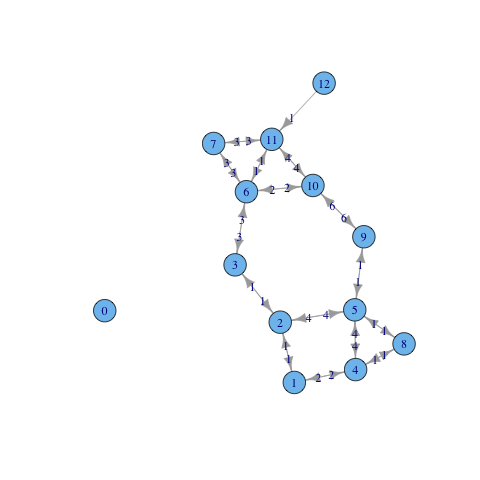
\includegraphics[scale=.5]{test_network.png} 
\caption{Lyhyimmän polun etsimiseen käytetty testiverkko}
\label{testiverkko}
\end{figure}

Täsmällisesti testit toteutettiin seuraaville tapauksille:

\begin{itemize}
\item Solmun 0 etäisyys kaikista muista solmuista tulee olla ääretön.
\item Kaikkien muiden solmujen etäisyys solmusta 0 tulee olla ääretön.
\item Etäisyys solmusta 12 solmuun 11 tulee olla 1.
\item Etäisyys solmusta 11 solmuun 12 tulee olla ääretön.
\item Lyhyin reitti solmusta 1 solmuun 5 kulkee solmujen 4 ja 8 kautta, ja muodostetun reitin pituus on 4.
\item Lyhyin reitti solmusta 5 solmuun 6 kulkee solmujen 2 ja 3 kautta, ja muodostetun reitin pituus on 8.
\item Lyhyin reitti solmusta 1 solmuun 11 kulkee solmujen 2, 3 ja 6 kautta, ja muodostetun reitin pituus on 6.
\item Lyhyin reitti solmusta 4 solmuun 5 kulkee solmun 8 kautta, ja muodostetun reitin pituus on 2.
\end{itemize}

Testit on toteutettu abstraktille yläluokalle \texttt{ShortestPathGraph}, jolloin samaa testikoodia voidaan käyttää sekä luokille \texttt{AStarPathGraph} sekä \texttt{DikstraPathGraph}.

\section{Evaluaatio}

\end{document}